% Comment to allow building from within this file
%!TEX root = pyconuk2016.tex

\blankscreen{
  Substance Paridigm\textCR
  \textCR
}

\begin{frame}{}

    \tikzstyle{primary} = [
        rectangle, rounded corners, line width=0.4mm, draw=blue,
        minimum height=2cm, minimum width=3cm, text width=3cm
    ]
    \tikzstyle{substance} = [
        rectangle, rounded corners, line width=0.4mm, draw=blue,
        top color=white, bottom color=blue!20,
        minimum height=2cm, minimum width=3cm
    ]
    \tikzstyle{attribute} = [
        rectangle, rounded corners, line width=0.4mm, draw=red,
        minimum width=2cm, fill=white, opacity=1
    ]
    \tikzstyle{hidden} = [
        rectangle, rounded corners,
        % line width=0.4mm, draw=green,
        minimum height=3cm, minimum width=6cm
    ]
    \tikzstyle{real} = [rectangle]
    \tikzstyle{line} = [line width=0.5mm]

    \begin{center}
        \resizebox{10cm}{!}{
            \begin{tikzpicture}
                \node[hidden](1) at (0, 9) {};
                    \node[hidden](2) at (-3, 6){};
                        \node[hidden](3) at (-3, 3){};
                            \node[hidden](4) at (-3, 0){};

                    \node[hidden](5) at (3, 6){};
                        \node[hidden](6) at (3, 3){};
                            \node[hidden](7) at (3, 0){};

                \node[hidden](8) at (9, 9){};
                    \node[hidden](9) at (9, 6){};
                        \node[hidden](10) at (9, 3){};
                            \node[hidden](11) at (9, 0){};


                \node<1->(real_mx5)[real] at (4){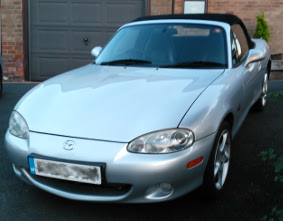
\includegraphics[width=3cm]{images/mx5}};

                \node<2->(real_mondeo)[real] at (7){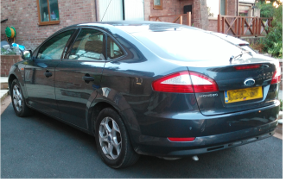
\includegraphics[width=3cm]{images/mondeo}};

                \node<3->(real_me)[real] at (11){
\includegraphics[width=3cm]{images/owencampbell}};

                \node<4->(my_mx5) at (3)[primary]{My\\ Toy Car};
                \draw<4->(real_mx5.north)--(my_mx5.south);

                \node<5->(my_mondeo) at (6)[primary]{My\\  Big Car};
                \draw<5->(real_mondeo.north) -- (my_mondeo.south);

                \node<6->(me) at (10)[primary]{Me};
                \draw<6->(real_me.north) -- (me.south);

                \node<7->(silver)[attribute] at (my_mx5.east){Silver};
                \node<7->(abc123)[attribute, anchor=north west] at (silver.south west){ABC 123};

                \node<8->(grey)[attribute] at (my_mondeo.east){Grey};
                \node<8->(xyz789)[attribute, anchor=north west] at (grey.south west){XYZ 789};

                \node<9->(owen)[attribute] at (me.east){Owen};
                \node<9->(1968)[attribute, anchor=north west] at (owen.south west){1968};

                \node<10->(mx5) at (2)[substance]{Mazda MX5};
                \draw<10->(my_mx5.north) -- (mx5.south);

                \node<11->(mondeo) at (5)[substance]{Ford Mondeo};
                \draw<11->(my_mondeo.north) -- (mondeo.south);

                \node<12->(person) at (9)[substance]{Person};
                \draw<12->(me.north) -- (person.south);

                \node<13->(car) at (1)[substance]{Car};
                \draw<13->(mx5.north) -- (car.south);
                \draw<13->(mondeo.north) -- (car.south);

            \end{tikzpicture}
        }
    \end{center}

\end{frame}
